\documentclass[12pt,compress,ngerman,utf8,t]{beamer}
\usepackage[english]{babel}
\usepackage{calc}
\usepackage{ragged2e,wasysym,multicol,mathtools}
\usepackage[protrusion=true,expansion=true]{microtype}
\hypersetup{colorlinks=true}

\graphicspath{{images/}}

\DeclareSymbolFont{extraup}{U}{zavm}{m}{n}
\DeclareMathSymbol{\varheart}{\mathalpha}{extraup}{86}

\title{Exploring hypercomputation \\ $\varheart$ with the ef{}fective topos $\varheart$}
\author[Ingo Blechschmidt]{\textcolor{white}{Ingo Blechschmidt \\ \scriptsize University of Augsburg \\ February 8th, 2017}}
\date[2017-02-08]{}

%\usetheme{Warsaw}
\useinnertheme[shadow=true]{rounded}
\useoutertheme{split}
\usecolortheme{orchid}
\usecolortheme{whale}
\setbeamerfont{block title}{size={}}

\useinnertheme{rectangles}

\usecolortheme{seahorse}
\definecolor{mypurple}{RGB}{150,0,255}
\setbeamercolor{structure}{fg=mypurple}
\definecolor{myred}{RGB}{150,0,0}
\setbeamercolor*{title}{bg=myred,fg=white}
\setbeamercolor*{titlelike}{bg=myred,fg=white}

\usefonttheme{serif}
\usepackage[T1]{fontenc}
\usepackage{libertine}
%\usepackage{mathpazo}

\renewcommand{\_}{\mathpunct{.}\,}
\newcommand{\BB}{\mathbb{B}}
\newcommand{\M}{\mathcal{M}}
\newcommand{\R}{\mathrm{R}}
\newcommand{\NN}{\mathbb{N}}
\newcommand{\RR}{\mathbb{R}}
\newcommand{\Eff}{\mathrm{Eff}}
\newcommand{\TM}{\mathrm{TM}}
\newcommand{\STM}{\mathrm{STM}}
\newcommand{\RW}{\mathrm{RW}}
\newcommand{\lambdaC}{\lambda\mathrm{C}}
\newcommand{\defeq}{\vcentcolon=}
\newcommand{\Set}{\mathrm{Set}}

\newcommand{\code}[1]{%
  \begin{center}%
    \setlength{\fboxrule}{1pt}%
    \setlength{\fboxsep}{8pt}%
    {\fbox{\parbox{0.81\textwidth}{#1}}}%
  \end{center}%
}

\newcommand{\explanation}[2]{
  #1 \\
  \qquad means: \\[0.4em]
  \qquad\qquad \begin{minipage}{0.84\textwidth}
  #2
  \end{minipage}
}

\newcommand{\explanationspoiler}[3]{
  \explanation{#1}{#2} \\[0.4em]
  \qquad\qquad\qquad #3
}

\newcommand{\fmini}[2]{%
  \setlength{\fboxrule}{2pt}%
  \setlength{\fboxsep}{-3pt}%
  \usebeamercolor[fg]{item}\fbox{\usebeamercolor[fg]{normal text}\parbox{#1}{\begin{center}#2\end{center}}}}

\setbeamertemplate{navigation symbols}{}

\setbeamertemplate{title page}[default][colsep=-1bp,rounded=false,shadow=false]
\setbeamertemplate{frametitle}[default][colsep=-2bp,rounded=false,shadow=false,center]

\newcommand{\hil}[1]{{\usebeamercolor[fg]{item}{\textbf{#1}}}}
\setbeamertemplate{frametitle}{%
  \vskip1em%
  \leavevmode%
  \begin{beamercolorbox}[dp=1ex,center]{}%
      \usebeamercolor[fg]{item}{\textbf{\Large \insertframetitle}}
  \end{beamercolorbox}%
}

\setbeamertemplate{footline}{%
  \leavevmode%
  \hfill%
  \begin{beamercolorbox}[ht=2.25ex,dp=1ex,right]{}%
    \usebeamerfont{date in head/foot}
    \insertframenumber\,/\,\inserttotalframenumber\hspace*{1ex}
  \end{beamercolorbox}%
  \vskip0pt%
}

\newcommand{\backupstart}{
  \newcounter{framenumberpreappendix}
  \setcounter{framenumberpreappendix}{\value{framenumber}}
}
\newcommand{\backupend}{
  \addtocounter{framenumberpreappendix}{-\value{framenumber}}
  \addtocounter{framenumber}{\value{framenumberpreappendix}}
}

\newcommand{\partslide}[5]{{\usebackgroundtemplate{\begin{minipage}{\paperwidth}\vspace*{#3}\centering\includegraphics[#2]{#1}\end{minipage}}
\begin{frame}
  \centering
  \bigskip\bigskip

  \Huge \hil{Part #4}

  \bigskip
  \Large\textbf{#5}
  \par
\end{frame}}}


\setbeameroption{hide notes}
\setbeamertemplate{note page}[plain]

\begin{document}

% http://www.ufointernationalproject.com/wp-content/uploads/2015/11/a23.jpg
{\usebackgroundtemplate{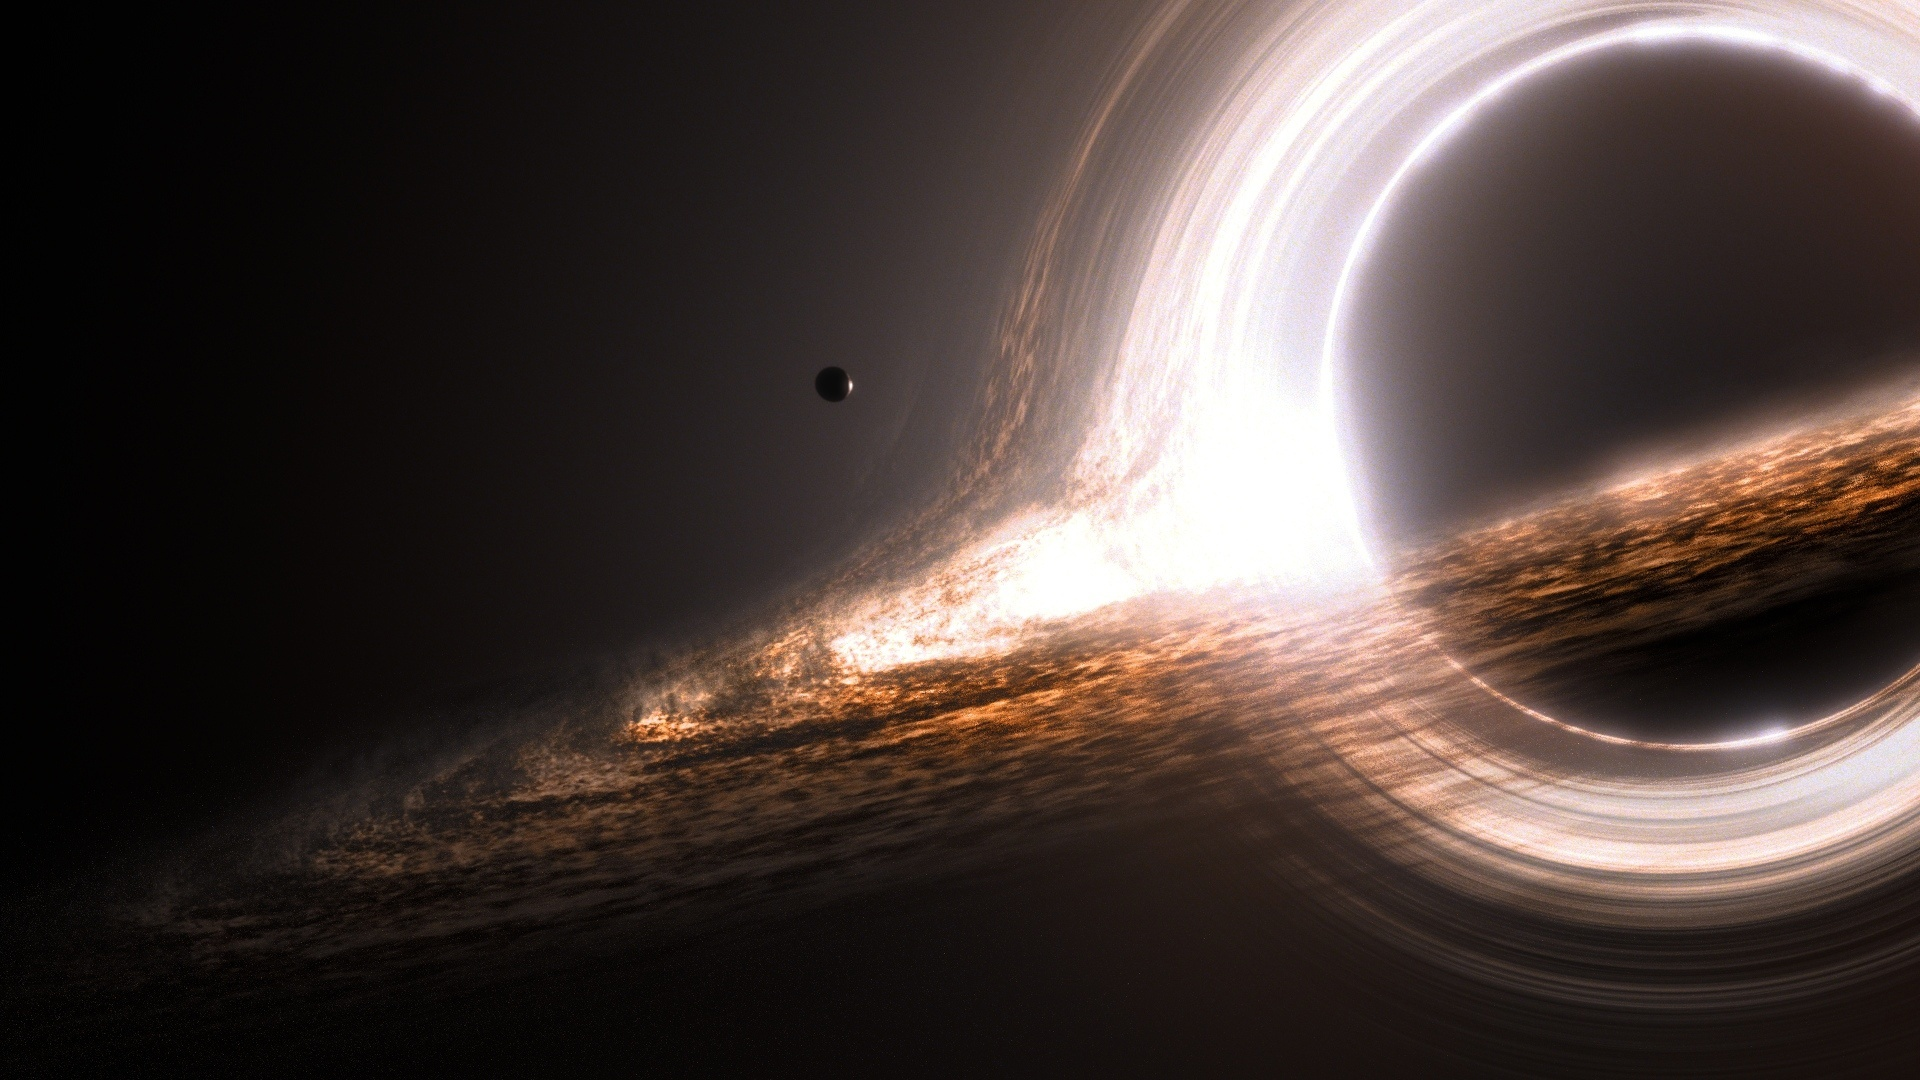
\includegraphics[height=\paperheight]{images/interstellar}}
\frame{\vspace*{11em}\titlepage}}
\setcounter{tocdepth}{2}
\frame{\tableofcontents}


\section[Ordinal numbers]{Crash course on ordinal numbers}

\partslide{infinite-queue}{width=0.4\paperwidth}{4.5cm}{I}{A crash course on ordinal numbers}


\section{(Super) Turing machines}

\partslide{turing-machine}{width=0.5\paperwidth}{4.5cm}{II}{(Super) Turing machines}


\subsection[TM]{Bacis on Turing machines}

\newcommand{\portrait}[4]{\begin{column}{#3\textwidth}\centering\includegraphics[height=#4\textheight]{#1}\\{\scriptsize #2\par}\end{column}}

\begin{frame}{Basics on Turing machines}
  \begin{itemize}
    \item Turing machines are idealised computers operating on an \hil{infinite
    tape} according to a \hil{finite list} of rules.
    \item The concept is astoundingly robust.
    \item A subset of~$\NN$ is \hil{enumerable by a Turing machine} if and only
    if it's a $\Sigma_1$-set.
  \end{itemize}

  \bigskip
  \begin{columns}[t]
    \begin{column}{0.095\textwidth}\end{column}
    \portrait{alan-turing}{Alan Turing \\ (* 1912, † 1954)}{0.27}{0.35}
    \portrait{imitation-game}{worth seeing}{0.27}{0.35}
    \portrait{alison-bechdel}{Alison Bechdel \\ (* 1960)}{0.27}{0.35}
    \begin{column}{0.095\textwidth}\end{column}
  \end{columns}
\end{frame}


\subsection[STM]{Bacis on super Turing machines}

\begin{frame}{Super Turing machines}
  With super Turing machines, the time axis is more interesting:
  \begin{itemize}
    \item normal: $0,\ 1,\ 2,\ \ldots$
    \item super:\phantom{rl} $0,\ 1,\ 2,\ \ldots,\ \omega,\ \omega + 1,\ \ldots,\ \omega\cdot2,\ \omega\cdot2
    + 1,\ \makebox[\widthof{R}][l]{$\ldots\ldots\ldots\ldots\ldots\ldots$}$
  \end{itemize}
  \bigskip

  On reaching a limit ordinal time step like~$\omega$ or~$\omega \cdot 2$,
  \begin{itemize}
    \item the machine is put into a designated state,
    \item the read/write head is moved to the start of the tape, and
    \item the tape is set to the ``lim sup'' of all its previous contents.
  \end{itemize}

  \bigskip
  \begin{columns}[t]
    \begin{column}{0.03\textwidth}\end{column}
    \portrait{joel-david-hamkins}{Joel David Hamkins}{0.23}{0.3}
    \portrait{mathoverflow}{MathOverflow}{0.38}{0.3}
    \portrait{phantom}{Andy Lewis}{0.23}{0.3}
    \begin{column}{0.03\textwidth}\end{column}
  \end{columns}
\end{frame}

{\usebackgroundtemplate{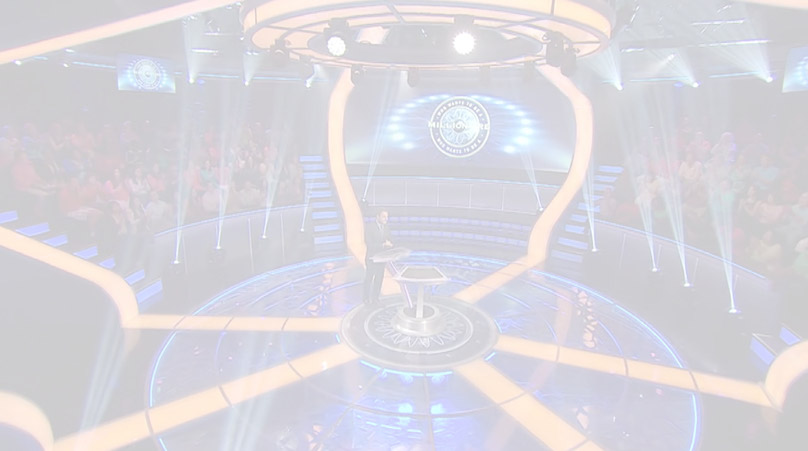
\includegraphics[height=\paperheight]{who-wants-to-be-a-millionaire}}
\begin{frame}{A question to you}
  \centering
  What's the behaviour of this super Turing machine?

  \code{In the start state and the limit state, check whether the current cell contains a ``1''.
  \begin{itemize}
    \item If yes, then stop.
    \item If not, then flash that cell: set it to ``1'', then reset it to ``0''. Then
    unremittingly move the head rightwards.
  \end{itemize}}
  \pause

  \parbox{0.72\textwidth}{\centering\hil{Super Turing machines can break out of (some kinds of) infinite loops.}\par}
  \par
\end{frame}}


\subsection[Power]{The power of super Turing machines}

\begin{frame}{What can super Turing machines do?}
  \begin{itemize}
    \item Everything ordinary Turing machines can do.
    \item Verify number-theoretic statements.
    \item Decide whether a given ordinary Turing machine halts.
    \item Simulate super Turing machines.
    \item Decide $\Pi_1^1$- and $\Sigma_1^1$-statements:
    \begin{itemize}
      \item ``For any function $\NN \to \NN$ it holds that \ldots''
      \item ``There is a function $\NN \to \NN$ such that \ldots''
    \end{itemize}
  \end{itemize}

  \visible<2>{\hil{But:} Super Turing machines can't calculate all functions
  and can't write all 0/1-sequences to the tape.}

  \begin{center}
    \scalebox{0.1}{\input{images/nonwellfounded-tree.pdf_t}}
  \end{center}
\end{frame}


\subsection[Outlook]{Outlook on the bigger theory}

{\usebackgroundtemplate{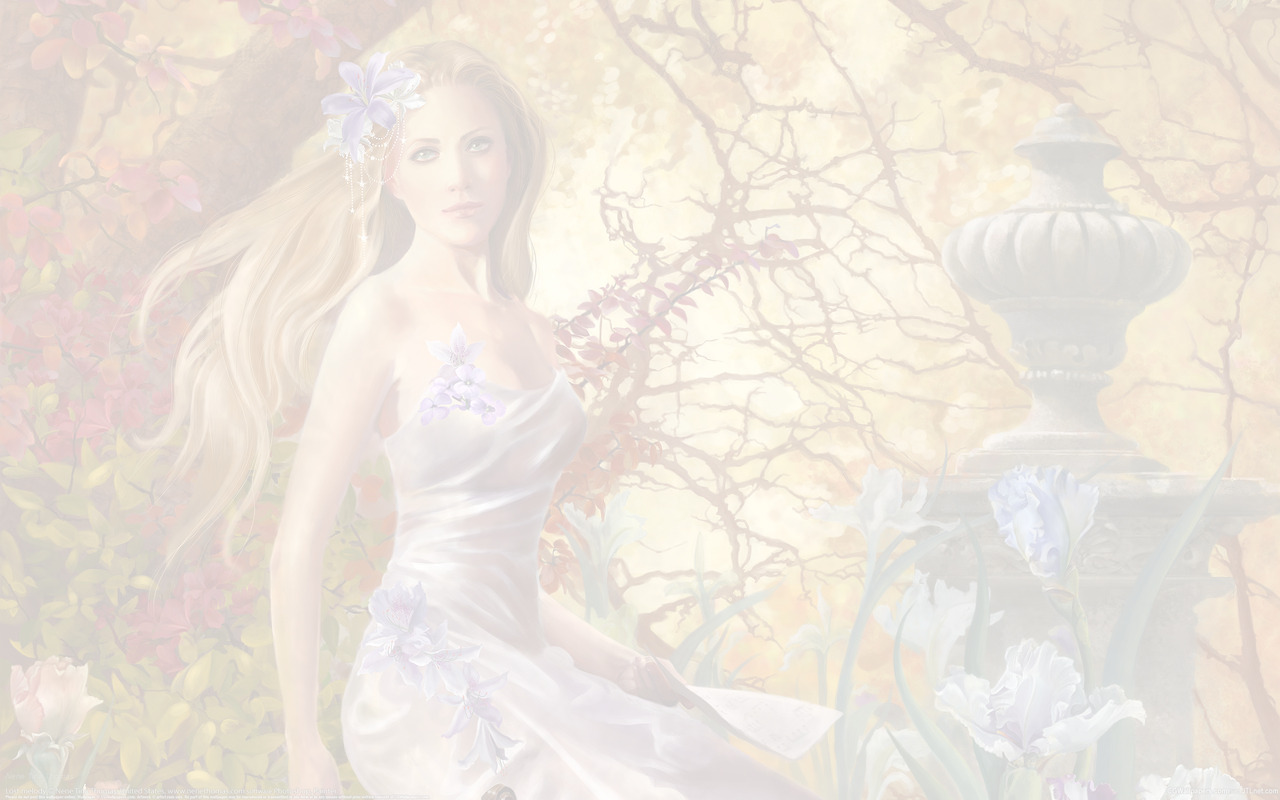
\includegraphics[height=\paperheight]{lost-melody}}
\begin{frame}{Fun facts}
  \begin{itemize}
    \item Any super Turing machine either halts or gets caught in an
    unbreakable infinite loop after \hil{countably many steps}.
    \item An ordinal number~$\alpha$ is \hil{clockable} iff there is a super
    Turing machine which halts precisely after time step~$\alpha$.
    \begin{itemize}
      \item Speed-up Lemma: If $\alpha + n$ is clockable, then so is $\alpha$.
      \item Big Gaps Theorem
      \item Many Gaps Theorem
      \item Gapless Blocks Theorem
    \end{itemize}
    \item \hil{Lost Melody Theorem:} There are 0/1-sequences which a super Turing
    machine can recognise, but not write to the tape.
  \end{itemize}
\end{frame}}


\section{The ef{}fective topos}

\partslide{topos-horses}{width=\paperwidth}{4.95cm}{III}{The ef{}fective topos}


\subsection[First steps]{First steps in the ef{}fective topos}

\begin{frame}{The ef{}fective topos}
  \begin{itemize}
    \item ``$1 + 1 = 2$.''

    \visible<2->{True in $\Set$, true in~$\Eff(\TM)$.}
    \medskip

    \item ``Any number is either prime or not.''

    \visible<3->{Trivially true in $\Set$, nontrivially true in~$\Eff(\TM)$.}
    \medskip

    \item ``Any function $\NN \to \NN$ is either the zero function or not.''

    \visible<4->{Trivially true in $\Set$, false in~$\Eff(\TM)$.}
    \medskip

    \item ``Any function $\NN \to \NN$ is computable by a Turing machine.''

    \visible<5->{False in $\Set$, trivially true in~$\Eff(\TM)$.}
    \medskip

    \item ``Any function $\RR \to \RR$ is continuous.''

    \visible<6->{False in $\Set$, true in~$\Eff(\TM)$.}
  \end{itemize}
\end{frame}

\begin{frame}{First steps in the ef{}fective topos}
  \small
  \explanation{$\Eff(\TM) \models \text{``For any number~$n$ there is a prime~$p
  > n$.''}$}{There is a Turing machine which reads a number~$n$ as input and outputs a
  prime number~$p > n$.}
  \bigskip

  \only<1>{
    \centering
    \hil{``Realisability Theory''}
    \par
  }
  \pause

  \explanation{\mbox{$\Eff(\TM) \models \text{``Any number has a prime factor
  decomposition.''}$}}{There is a Turing machine which reads a number $n$ as input and
  outputs a list of primes, the product of which is~$n$.}
  \bigskip
  \pause

  \explanation{$\Eff(\TM) \models \text{``Any number is either prime or not
  prime.''}$}{There is a Turing machine which reads a number $n$ as input and outputs
  YES or NO depending on whether $n$ is prime or not.}
\end{frame}


\subsection[Constructive logic]{The wonder of constructive logic}

\subsubsection{What's true in alternate toposes?}

\begin{frame}{What's true in alternate toposes?}
  \hil{Metatheorem:} If a statement has a \hil{constructive proof},
  then it holds in \hil{any topos}.
  \bigskip

  Constructive logic is like classical logic, except we don't suppose the
  \hil{law of excluded middle} (LEM), which says:
  \begin{itemize}
    \item ``Any statement is either true or not true.''
    \item ``If a statement is \emph{not not} true, then it's true.''
  \end{itemize}

  \bigskip\centering
  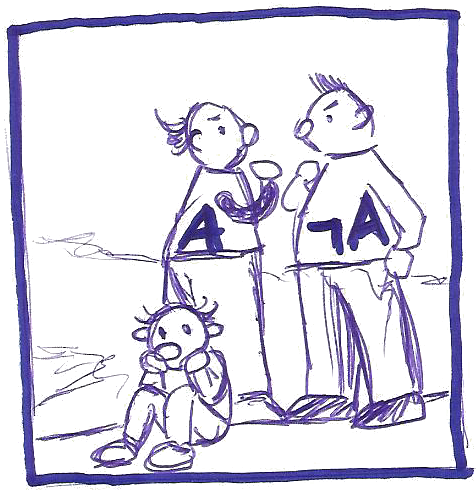
\includegraphics[width=0.2\textwidth]{images/lem}
  \par
\end{frame}


\subsubsection{Nonconstructive proofs}

\begin{frame}{Nonconstructive proofs}

  {\centering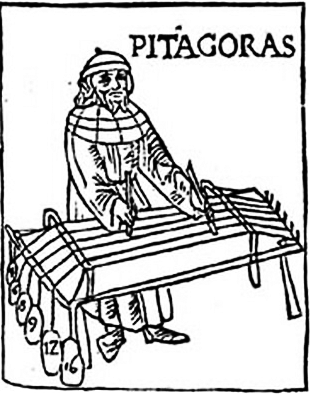
\includegraphics[scale=0.20]{pythagoras}\par}

  \hil{Theorem.} There are \hil{irrational} numbers~$x$ und~$y$ such that~$x^y$ is rational.
  \medskip

  \pause
  \hil{Proof.} Either~$\sqrt{2}^{\sqrt{2}}$ is rational or not.
  \begin{enumerate}
    \item In the first case we are done.
    \item In the second case we set~$x \defeq \sqrt{2}^{\sqrt{2}}$ and~$y \defeq
    \sqrt{2}$. Then~$x^y = \sqrt{2}^{\sqrt{2} \cdot \sqrt{2}} =
    \sqrt{2}^2 = 2$ is rational.
  \end{enumerate}
\end{frame}


\subsubsection[Praise]{Appreciating constructive logic}

\begin{frame}{Appreciating constructive logic}
  At first sight, dropping the axiom of excluded middle looks like a sad thing
  to do. It's a useful axiom! However:

  \begin{itemize}\justifying
    \item The axiom is not needed as often as one would think.
    \item The abstinence is good for your mental hygiene.
    \item Constructive logic allows for finer distinctions.
    \item From constructive proofs one can mechanically extract programs which
    witness the proved statements.
    \item \hil{Dropping the law of excluded middle allows to add curious unconvential axioms.}
  \end{itemize}
\end{frame}


\subsection[Tautologies]{Ef{}fective content of classical tautologies}

\subsubsection[Functions]{Equality of functions}

\begin{frame}{LEM for equality of functions}
  \explanationspoiler{$\Eff(\TM) \models \begin{minipage}[t]{0.7\textwidth}
  ``Any function~$f : \NN \to \NN$ is either the zero function or
  not.''\\[-0.7em]\end{minipage}$}{There is a Turing machine which reads the
  source of a Turing machine~$M$, which calculates a function $\NN \to \NN$, as input, and finds out whether~$M$ always yields zero or not.}{That's false.}
  \bigskip
  \pause

  The statement is true in~$\Eff(\STM)$, the ef{}fective topos associated to
  super Turing machines.
\end{frame}


\subsubsection[Halting]{The halting problem}

\begin{frame}{LEM for the halting problem}
  \explanationspoiler{$\Eff(\TM) \models \text{``Any Turing machine halts or
  doesn't halt.''}$}{There is a Turing machine which reads the source of a Turing machine~$M$
  as input and finds out whether $M$ halts or not.}{That's false.}
  \bigskip
  \pause

  The statement is true in~$\Eff(\STM)$.
\end{frame}


\subsubsection[Reals]{Equality of real numbers}

\begin{frame}{LEM for equality of real numbers}
  \justifying
  The statement
  \[ \text{``Every real number is either zero or not zero.''} \]
  is in constructive logic equivalent to
  \[ \text{``Every Turing machine halts or doesn't halt.''}, \]
  so it's not true in~$\Eff(\TM)$, but in~$\Eff(\STM)$.
  \bigskip
  \pause

  For a Turing machine~$M$ consider the real number~$0.000\ldots$ whose~$n$'th
  decimal digit is a one iff~$M$ halts after step~$n$.
  \bigskip

  For a real number~$x$ consider the Turing machine which searches the digits
  of~$x$ for a nonzero digit.
  \par
\end{frame}

\note{\justifying
  Stimmt die Aussage in~$\Eff(\RW)$, dem effektiven Topos zu Maschinen der
  realen Welt? Das heißt: Ist es möglich, in der realen Welt ein Halteorakel zu
  bauen? Also eine Maschine, welche die Beschreibung einer Turingmaschine einliest
  und dann korrekt ausgibt, ob die Turingmaschine hält oder nicht?
  \bigskip

  Da es hier nicht um das Halteproblem für Maschinen der realen Welt geht
  (welches für Maschinen der realen Welt wegen des üblichen Arguments nicht
  entscheidbar ist), sondern nur um das Halteproblem für Turingmaschinen, ist
  die Antwort "`ja"' nicht prinzipiell ausgeschlossen. Vielleicht sind Tricks
  mit schwarzen Löchern und relativistischer Zeitdilatation möglich.
  \par
}


\subsubsection[Markov]{Markov's principle}

\begin{frame}{Markov's principle}
  \explanationspoiler{$\Eff(\TM) \models \begin{minipage}[t]{0.7\textwidth}
  ``For any function~$f : \NN \to \NN$ which is not the zero function,
  there is a number~$n \in \NN$ such that~$f(n) \neq
  0$.''\\[-0.7em]\end{minipage}$}{There is a Turing machine which reads the source of a
  Turing machine~$M$, which calculates a function~$\NN \to \NN$ which is not the zero
  function, as input and outputs a number~$n$ such that~$M(n)$ is not
  zero.}{\pause That's true! By unbounded search.}
\end{frame}


\subsubsection[Imp.\@]{Searching uncountable sets}

\begin{frame}{Searching uncountable sets}
  \begin{center}\parbox{0.91\textwidth}{
    ``For any function $f : \NN \to \NN$ from numbers to numbers,
    there either exists a number~$n$ such that $f(n)$ is one or there is no such number.''
  }\end{center}
  This statement is false in~$\Eff(\TM)$.
  \bigskip
  \bigskip

  \begin{center}\parbox{0.91\textwidth}{
    ``For any function $P : L(\BB) \to \BB$ from infinite lists of booleans to booleans,
    there either exists a list~$x$ such that $P(x)$ is true or there is no such list.''
  }\end{center}
  \pause
  This statement is true in~$\Eff(\TM)$!
\end{frame}


\subsubsection[Church--Turing]{The Church--Turing thesis}

\begin{frame}{The Church--Turing thesis}
  \justifying
  The \hil{Church--Turing thesis} states:
  \bigskip

  {\centering\parbox{0.8\textwidth}{If a function $f : \NN \to
  \NN$ is calculable in the real world, then it's also calculable by a Turing
  machine.}\par}
  \bigskip

  \explanationspoiler{$\Eff(\TM) \models \begin{minipage}[t]{0.7\textwidth}
  ``Any function~$f : \NN \to \NN$ is calculable by a
  Turing machine.''\\[-0.7em]\end{minipage}$}{There is a Turing machine which reads the source of a
  Turing machine calculating a function~$f : \NN \to \NN$ as input and
  outputs the source of a Turing machine which calculates~$f$.}{That's trivial,
  echo the input back to the user.}
  \bigskip
  \pause

  In~$\Eff(\STM)$ the statement is false.
\end{frame}

\note{\justifying
  Der effektive Topos zu Turingmaschinen ist also eine schöne Umgebung für die
  Informatik, da in ihm \emph{jede Funktion~$\NN \to \NN$ berechenbar ist} und
  unberechenbare Funktionen aussortiert wurden.
  \bigskip

  Vielleicht vermutet man hierbei einen Widerspruch. Sind nicht etwa folgende
  Funktionen unberechenbar? Was verhindert ihre Existenz im effektiven Topos?
  \begin{align*}
    H(n) &= \begin{cases}
      1, & \text{falls die~$n$-te Turingmaschine hält,} \\
      0, & \text{sonst.}
    \end{cases} \\
    BB(n) &= \text{höchste Anzahl Schritte, die eine haltende Turingmaschine} \\
    &\qquad\quad \text{mit~$n$ Zuständen durchführt, bevor sie hält.}
  \end{align*}

  Um zu zeigen, dass~$H$ und~$BB$ beides totale Funktionen~$\NN \to \NN$ sind
  -- und nur auf solche bezieht sich die Church--Turing-These --, ist LEM nötig!
  Für~$H$, damit die Fallunterscheidung getroffen werden kann. Für~$BB$, weil
  implizit das Lemma verwendet wurde, dass eine subendliche Menge natürlicher
  Zahlen ein größtes Element enthält.\par
}

\note{\justifying
  Die Aussage, dass \emph{jede} Funktion~$\NN \to \NN$ durch eine
  Turingmaschine berechenbar ist, ist auch als \emph{formale
  Church--Turing-These} bekannt.
  \begin{itemize}
    \item\justifying In~$\Eff(\STM)$ gilt sie nicht, denn aus einer
    Superturingmaschine, welche eine Funktion~$\NN \to \NN$ berechnet, kann man
    nur in den seltensten Fällen in eine gewöhnliche Turingmaschine mit
    demselben Ausgabeverhalten umwandeln.
    \item In~$\Eff(\lambdaC)$ gilt die formale Church--Turing-These ebenfalls
    nicht, aber aus einem anderen Grund. Die These lautet in diesem Fall:
    \begin{center}\parbox{0.83\textwidth}{
      Es gibt einen~$\lambda$-Term~$T$, sodass für jeden~$\lambda$-Term~$u$,
      welcher eine Funktion~$f : \NN \to \NN$ berechnet, der~$\lambda$-Term~$T\ u$
      die Kodierung einer Turingmaschine ist, welche~$f$ berechnet.
    }\end{center}
    Der ominöse Term~$T$ kann sein Argument~$u$ nur auf Eingaben auswerten, er
    hat aber keinen Zugriff auf die syntaktische Struktur von~$u$.
    (Konventionsgemäß werden in~$\Eff(\TM)$ Turingmaschinen höherer Ordnung
    dadurch realisiert, dass sie als Argument Kodierungen von
    Turingmaschinen erhalten. Beim~$\lambda$-Kalkül ist der Umweg über
    syntaktische Kodierungen nicht nötig und wird in~$\Eff(\lambdaC)$ auch
    nicht verfolgt.)
  \end{itemize}
}


\subsubsection[Cont.\@]{Automatic continuity}

\begin{frame}{Automatic continuity}
  \justifying
  The following statement is wildly \hil{false} in~$\Set$:
  \[ \text{``Every function $f : \RR \to \RR$ is continuous.''} \]
  A function~$f$ is \hil{continuous} if and only if, for calculating~$f(x)$ to
  finitely many digits, finitely many digits of~$x$ suffice.\par

  \centering
  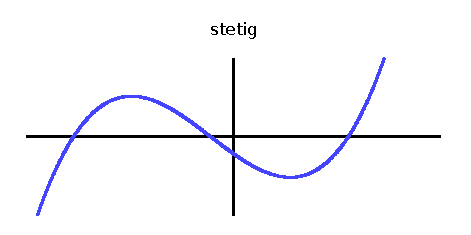
\includegraphics[width=0.5\textwidth]{images/plot-1}
  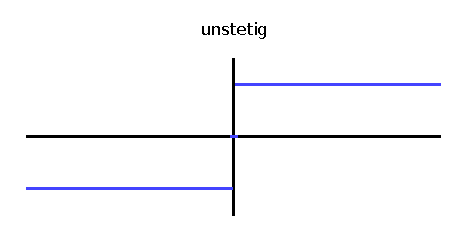
\includegraphics[width=0.5\textwidth]{images/plot-2}
  \par
  \pause

  \justifying
  \hil{True} in $\Eff(\TM)$. \pause
  True in~$\Eff(\RW)$, if private communication channels are possible and
  only finitely many computational steps can be executed in finite time.\par
\end{frame}

\note{\justifying
  Gibt es nicht offensichtlich unstetige Funktionen? Wie etwa die
  Signumfunktion?
  \[ \mathrm{sgn} : \RR \to \RR, \quad
    x \mapsto \begin{cases}
      -1, & \text{falls $x < 0$,} \\
      0,  & \text{falls $x = 0$,} \\
      1,  & \text{falls $x > 0$.}
    \end{cases}
  \]
  Ohne Verwendung von LEM ist die Situation nicht so trivial. Ohne es kann man
  nämlich nicht zeigen, dass diese Zuordnung eine auf ganz~$\RR$ definierte
  Funktion definiert: Dazu benötigte man das Lemma, dass jede reelle Zahl
  kleiner, gleich oder größer als Null ist. Dieses Lemma impliziert aber die
  schwächere Aussage, dass jede reelle Zahl gleich Null oder ungleich Null ist.
  Wir haben schon gesehen, dass diese Aussage in~$\Eff(\TM)$ nicht stimmt.
  \medskip

  Ohne LEM definiert obige Zuordnung nur eine Funktion~$M \to \RR$, wobei~$M =
  \{ x \in \RR \,|\, x < 0 \vee x = 0 \vee x > 0 \}$. Über solche Funktionen
  geht es hier aber nicht.
  \par
}

\note{\justifying
  Die in der Mathematik üblichen Definitionen des Konzepts reeller Zahlen sind
  in~$\Eff(\TM)$, $\Eff(\STM)$ und~$\Eff(\RW)$ alle zueinander äquivalent
  (obwohl sie es unter bloßer Verwendung von intuitionistischer Logik nicht
  sind).\bigskip

  Aus externer Sicht ist eine reelle Zahl in jedem der drei Fälle durch
  eine Maschine gegeben, die in sich konsistente, beliebig genaue
  Approximationen produziert. Etwa kann man eine solche Maschine nach
  Approximationen auf drei, sieben und zehn Ziffern fragen und die Antworten
  \[ 3.1417777777, \quad 3.1415926777 \quad\text{und}\quad 3.1415926535 \]
  erhalten.
  \bigskip

  Maschinen, welche andere, aber genauso gute Approximationen
  liefern, stellen dieselbe reelle Zahl dar.\par
}

\note{\justifying\footnotesize
  Die Aussage~"`Alle Funktionen~$\RR \to \RR$ sind stetig."' des effektiven
  Topos bedeutet: Es gibt eine Maschine~$M$, die
  \begin{enumerate}
    \item\justifying eine Maschine~$A$, welche eine Funktion~$f : \RR \to \RR$
    berechnet,
    \item eine Maschine~$X$, welche eine reelle Zahl~$x$ repräsentiert, sowie
    \item eine natürliche Zahl~$n$
  \end{enumerate}
  als Argumente nimmt und eine natürliche Zahl~$m$ mit folgender Eigenschaft
  ausgibt: Für jede reelle Zahl~$\tilde x$, deren erste~$m$ Ziffern mit denen
  von~$x$ übereinstimmen, stimmen die ersten~$n$ Ziffern von~$f(x)$ mit denen
  von~$f(\tilde x)$ überein.\smallskip

  Im Fall der realen Welt kann man wie folgt versuchen, eine derartige
  Maschine~$M$ zu konstruieren. Gegeben~$A$, $X$ und~$n$, wendet sie~$A$ auf
  eine leichte Variante~$X'$ von~$X$ an: Die Maschine~$X'$ soll dasselbe
  Ausgabeverhalten zeigen wie~$X$, allerdings bei jedem Aufruf über einen
  privaten Kommunikationskanal an~$M$ die Information übermitteln, wie viele
  Stellen abgefragt wurden. Da~$X'$ dasselbe Ausgabeverhalten wie~$X$ zeigt,
  muss~$A$ per Vertrag auf~$X'$ genauso reagieren wie auf~$X$.\smallskip

  Wenn nun in endlicher Zeit nur endlich viele Rechenschritte durchführbar sind, so
  muss~$M$ nur warten, bis~$A$ die Zahl~$f(x)$ auf~$n$ Stellen genau berechnet
  hat, und kann dann nachsehen, wie viele Stellen~$A$ für diese Berechnung
  benötigt hat. Für jede andere Zahl, die~$x$ in diesen Stellen gleicht,
  produziert somit~$A$ dieselben~$n$ Ziffern.\par
}

\note{\justifying
  Kein Fan von reellen Zahlen? Dasselbe Phänomen zeigt sich auch bei Funktionen
  von anderen Typen. Zum Beispiel für Funktionen~$f : \BB^\NN \to \BB$. Dabei
  ist~$\BB = \{ 0, 1 \}$ die Menge der Bools. Eine solche Funktion heißt genau
  dann \emph{stetig}, wenn es für jedes Argument~$x \in \BB^\NN$ (also jede
  Funktion~$x : \NN \to \BB$) eine natürliche Zahl~$m$ gibt, sodass~$f(x)$ nur
  von den ersten~$m$ Funktionswerten von~$x$ abhängt.\bigskip

  In~$\Eff(\TM)$ stimmt es, dass jede solche Funktion~$f$ stetig ist. Das ist
  der tiefere Grund dafür, wieso die "`scheinbar unmöglichen
  Haskell-Programme"' funktionieren.\par
}


\subsection{Wrapping up}

{\usebackgroundtemplate{\begin{minipage}{\paperwidth}\vspace*{4.95cm}\centering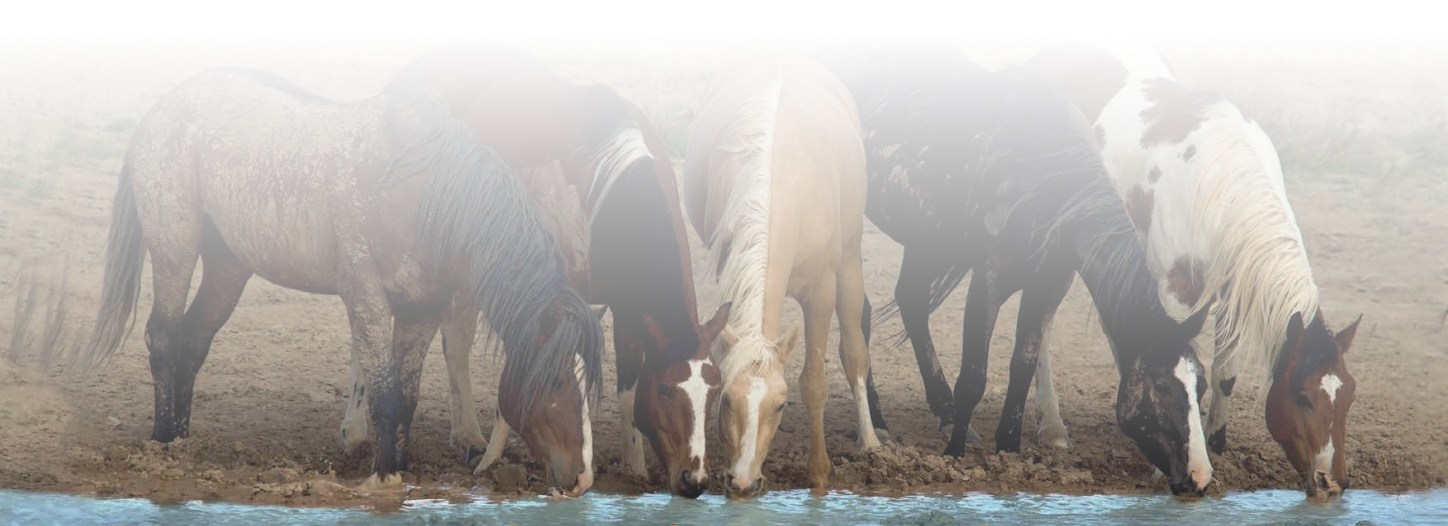
\includegraphics[width=\paperwidth]{topos-horses}\end{minipage}}
\begin{frame}{Wrapping up}
  \begin{itemize}
    \item Ef{}fective toposes are a good vehicle for studying the nature of computation.
    \item The ef{}fective toposes build links between constructive mathematics and programming.
    \item Toposes allow for curious dream axioms.
    \item Toposes also have a geometric flavour: points, subtoposes, maps
    between toposes.
  \end{itemize}
  \pause

  \centering
  \bigskip
  \hil{\textcolor{white}{There is more to mathematics \\
  than the standard topos.}}
  \par
\end{frame}}

\end{document}
